\chapter{Исследование функций с помощью производных.}
\section{Монотонность. Локальный экстремум}
$ f : |a;b| \rightarrow \Rm$\\\\
Вспомним, что означает, что $f$ монотонна на $|a;b|$\\\\
$\forall x_1,x_2 \in |a;b|$, \begin{center}$x_1 < x_2 \Rightarrow f(x_1) < f(x_2)$ -- строго возрастает\\
	$x_1 < x_2 \Rightarrow f(x_1) \le f(x_2)$ -- возрастает\\
	$x_1 > x_2 \Rightarrow f(x_1) > f(x_2)$ -- строго убывает\\
	$x_1 < x_2 \Rightarrow f(x_1) \ge f(x_2)$ -- убывает\\
\end{center}
\begin{theorem}[Критерий монотонности диффиренцируемой функции] Пусть $f \in \mathcal{C} ([a;b]) \wedge f \in D(]a;b[)$. Тогда для монотонности $f$ на $[a;b]$ необходимо и достаточно, чтобы $f^\prime$ не меняла знак на интервале $]a;b[$. При этом для возрастания $f$ необходимо и  достаточно $f^\prime(x) \ge 0$, для убывания -- $f^\prime(x) \le 0$ на интервале $]a;b[$. 
\end{theorem}
\begin{Proof}
	(Для возрастающей функции)\\
	\textbf{Необходимость}. $f$ возрастает. Докажем, что $f^\prime (x) \ge 0$ на $]a;b[$.\\\\ Рассмотрим $\Delta f = f(x + \Delta x) - f(x) \ge 0$ если  $\Delta x > 0$ и $\Delta f \le 0$, если $\Delta x < 0$ на основании того, что $f$ возрастает. В любом случае $\frac{\Delta f}{\Delta x} \ge 0$. Поэтому для $\forall x \in ]a;b[$, $\forall \Delta x$; $x + \Delta x \in ]a;b[ \Rightarrow \lim\limits_{x \rightarrow 0}\frac{\Delta f}{\Delta x} \ge 0 \Rightarrow f^\prime(x) \ge 0$.\\\\
	\textbf{Достаточность}.  $f^\prime(x) \ge 0$, $\forall x \in ]a;b[$. Докажем, что $f$ возрастает.\\\\ Для $\forall x_1,x_2 \in [a;b]$ по формуле конечных приращений $f(x_1) - f(x_2) = f^\prime(c)(x_1 - x_2)$. И если $x_1 < x_2 \Rightarrow f(x_1) - f(x_2) \le 0 \Rightarrow f(x_1) \le f(x_2)$, так как $^f\prime(c) \ge 0 \Rightarrow f$ возрастает.\\\\
	Для убывающей функции доказывается аналогично.
\end{Proof}
\begin{corollary}[Критерий строгой монотонности дифференцируемой функции] Пусть $f \in \mathcal{C} ([a;b]) \wedge f \in D(]a;b[)$. Для строгой монотонности $f$ на $[a;b]$ необходимо и достаточно, чтобы $f^\prime$ не меняла знак на интервале $]a;b[$ и необращалась  тождественно в нуль ни на одном интервале из $]a;b[$.
\end{corollary}
\begin{Proof}
	\textbf{Необходимость}. Дано: $f$ строго возрастает. Требуется доказать: $f^\prime(c) \ge 0$ и $f \not\equiv 0$ $]\alpha;\beta[$. Так как $f$ строго возрастает, то нет участников постоянства и по критерию постоянства дифференцируемой функции $\Rightarrow f^\prime(x) \not\equiv 0$, но $f^\prime(x) \ge 0$.\\\\
	\textbf{Достаточность}. $f^\prime(x) \ge 0$ и $f^\prime(x) \not\equiv 0$, то есть $f$ возрастает и нет участников постоянства $\Rightarrow$ $f$ строго возрастает.
\end{Proof}\\\\
\textbf{Замечание}.
\begin{enumerate}
	\item Всё справедливо, если $[a;b] \leftrightarrow |a;b|$
	\item У сторого монотонной функции производная может обращаться в нуль в отдельный точках. Например, $y = x^3$.
\end{enumerate}
\subsection{Необходимые условия локального экстремума.}
$I:: = |a;b|$, $f: I \rightarrow \Rm$.
Внутренняя точка $x_0 \in I$ называется точкой локального экстремума функции $f$, если $\exists U(x_0) \subset I$, на которой $x_0$ является точкой экстремума (обычно, глобального) для функции $f$, то есть
$\forall x \in U(x_0)$
$\begin{matrix}
	f(x) \le f(x_0) \Ra x_0\text{ --- точка максимума}; \\
	f(x) \ge f(x_0) \Ra x_0\text{ --- точка минимума}.
\end{matrix}$\\\\
На основании теоремы Ферма точками локального экстремума функции $f$ непрерывной на $[a;b]$ и дифференцируемой на $]a;b[$ могут быть только стационарные точки, то есть точки, в которых $f\prime(x) = 0$.\\\\
Действительно, если $x_0$ --- точка локального экстремума, то $\exists U(x_0)$, что $\forall x \in U(x_0)$ $f(x) \le f(x_0)$ (или $f(x) \ge f(x_0)$).\\\\
Применяя теорему Ферма на $U(x_0)$ заключаем, что $f^\prime(x) = 0$. Таким образом, немножечко подумав, приходим к 
\begin{theorem}[Необходимое условие локального максимума]
	Для того, чтобы точка $x_0$ была точкой локального экстремума функции $f : u(x_0) \rightarrow \Rm$, определённой в окрестности этой точки, необходимо выполнение одного из двух условий:
	\begin{enumerate}
		\item функция недифференцируема в точке $x_0$
		\item $x_0$ стационарная точка  функции $f$ 
	\end{enumerate}
\end{theorem}
$\bullet$ \textit{Все эти точки будем называть \textbf{критическими точками} либо 
	\textbf{точками возможного экстремума}.}
\subsection{Достаточные условия локального экстремума дифференцируемой функции} 
Есть несколько правил выполнения того, будет ли в критической точке $x_0$ локальный экстремум
\begin{enumerate}
	\item \begin{theorem}
		Пусть $f: U(x_0) \rightarrow \Rm$ --- функция, определённая в окрестности критической точки $x_0$, непрерывная на $U(x_0)$ и дифференцируемая на $U(x_0)$.\\\\
		Пусть\\ $\dot U_-(x_0) = \{x\ |\ x \in U(x_0), x < x_0\}$\\
		$\dot U_+(x_0) = \{x\ |\ x\in U(x_0), x > x_0\}$\\\\
		Тогда, если $f^\prime$ на $\dot U_-(x_0)$ и $\dot U_+(x_0)$ имеет разные знаки, то $x_0$ --- точка локального экстремума. Причём, если при переходе через точку $x_0$ $f^\prime$ меняет знак с $\oplus$ на $\circleddash$, то $x_0$ --- точка локального максимума; если при переходе через точку $x_0$ $f^\prime$ меняет знак с $\circleddash$ на $\oplus$, то $x_0$ -- точка локального минимума.\\\\
		Если же $f^\prime$ на $\dot U_-(x_0)$ и $\dot U_+(x_0)$ имеет одинаковые знаки, то $x_0$ не является точкой локального экстремума (либо строго убывает, либо строго возрастает).\\\\
		Знак $f^\prime$
		\begin{center}
			\begin{tabular}{c|c|c}
				$x < x_0$ & $x > x_0$ & \\
				\hline
				$+$ & $-$ & $\max$  \\
				\hline
				$-$ & $+$ & $\min$ \\
				\hline
				$+$ & $+$ & экстремума нет  \\
				\hline
				$-$ & $-$ & экстремума нет  \\
			\end{tabular}
		\end{center}
		$$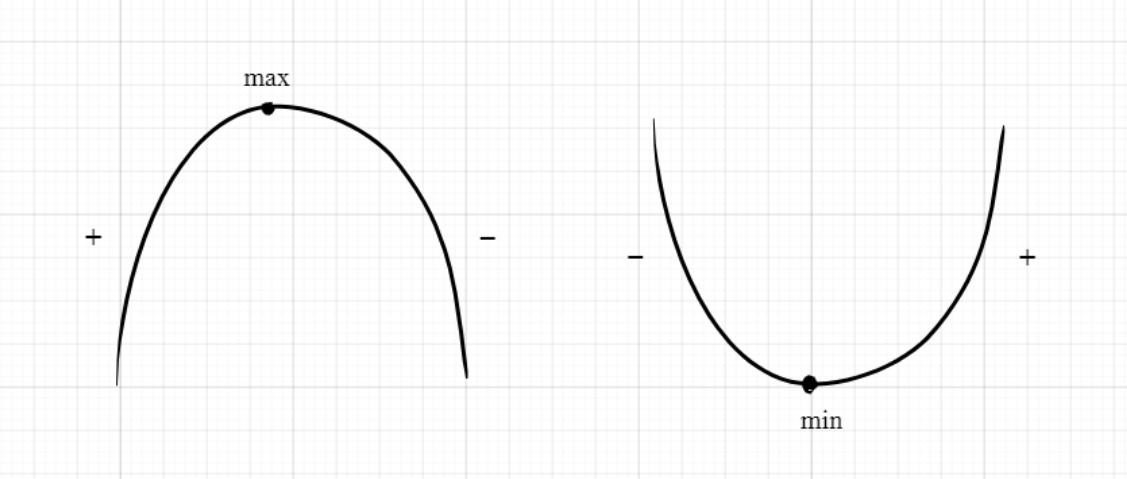
\includegraphics[scale=0.5]{images/img28.png}$$
	\end{theorem}
	\begin{Proof}
		\begin{enumerate}
			\item Если $f^\prime$ не меняет знака при переходе через точку $x_0$. Например, $+$ и $+$. Тогда на $\dot U_-(x_0) f$ строго возрастает. Так как в $x_0$ она не прерывна, то $f(x_0 - 0) = f(x_0)$ и, следовательно $f(x) < f(x_0)$ при $x \in \dot U_-(x_0)$. Аналогично $f(x) > f(x_0)$ при $x \in \dot U_+(x_0)$. Таким образом, $f$ строго возрастает во всей окрестности  точки $x_0$ и $x_0$ не является точкой экстремума.
			\item Пусть $f$ меняет знак с $\oplus$ на $\circleddash$. Тогда на $\dot U_-(x_0) f$ строго возрастает и $f(x) < f(x_0)$; на $\dot U_+(x_0) f$ строго убывает и $f(x) < f(x_0)$ $\Rightarrow x_0$ -- точка строгого локального максимума.
		\end{enumerate}
		Остальные случаи рассматриваются аналогично.
	\end{Proof} 
	\item \begin{theorem}
		Пусть $f: U(x_0) \rightarrow \Rm$ определённая в окрестности точки $x_0$, дважды дифференцируемая в точке $x_0$, $f^\prime(x_0) = 0$, а $f^{\prime\prime}(x_0) \neq 0$. Тогда, если $f^{\prime\prime}(x_0) > 0$, то $x_0$ -- точка локального минимума, если $f^{\prime\prime}(x_0) < 0$, то $x_0$ -- точка локального максимума.
	\end{theorem}
	\begin{Proof}
		Воспользуемся формулой Тейлора-Пеано второго порядка $$f(x) = f(x_0) + \frac{f^\prime(x_0)}{1!} (x - x_0) + \frac{f^{\prime\prime}(x_0)}{2} {(x - x_0)}^2 + o({(x - x_0)}^2).$$
		Перепишем эту формулу в виде
		$$f(x) - f(x_0)  = (\frac{f^{\prime\prime}(x_0)}{2} + o(1)) {(x - x_0)}^2$$
		Так как $f^{\prime\prime}(x_0) \neq 0$, то при $x$ достаточно близких к $x_0$ знак $\frac{f^{\prime\prime}(x_0)}{2} + o(1)$ совпадает со знаком $f^{\prime\prime}(x_0)$.\\\\
		Так как ${(x - x_0)}^2 \ge 0$ для $\forall x \in U(x_0)$, то $\frac{f^{\prime\prime}(x_0)}{2} + o(1)) {(x - x_0)}^2$ имеет такой знак, как и $f^{\prime\prime}(x_0)$. Поэтому  при $f^{\prime\prime}(x_0) > 0 \Rightarrow f(x) - f(x_0) \ge 0 \Rightarrow f(x) \ge f(x_0)$, то есть $x_0$ -- точка минимума. Если же $f^{\prime\prime}(x_0) < 0 \Rightarrow f(x) \le f(x_0) \Rightarrow$ $x_0$ --- точка максимума.  
	\end{Proof} \\\\
	Правило 2 еще называют правилом дождика или критерием рюмки.
	$$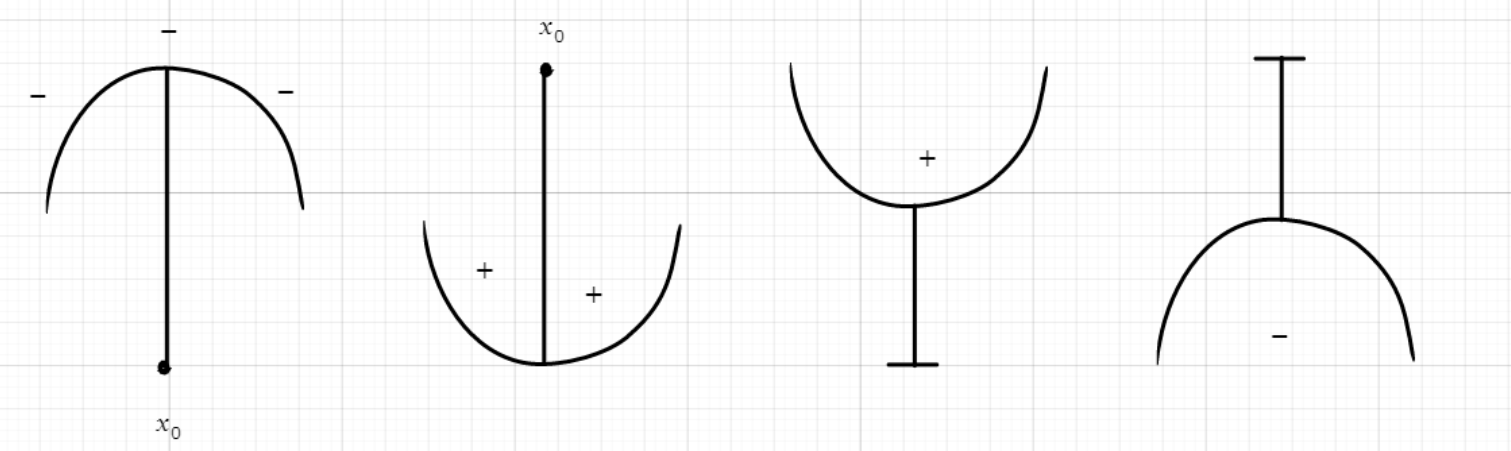
\includegraphics[scale=0.5]{images/img30.png}$$
	\item \begin{theorem}[Является обобщением правила 2]
		Пусть $f: U(x_0) \rightarrow \Rm$ определённая в окрестности точки $x_0$ и имеет в точке $x_0$ производные до порядка $n$ включительно $(n \ge 1)$ и $f^\prime(x_0) = f^{\prime\prime}(x_0) = \dots = f^{(n - 1)}(x_0) = 0$, а $f^{(n)}(x_0) \neq 0$. Тогда при нечётном $n$ локального экстремума в точке $x_0$ нет. Если же $n$ чётно, то локальный экстремум есть. При этом, если $f^{(n)}(x_0) \ge 0$ -- локальный минимум, если , то $x_0$ $f^{(n)}(x_0) \le 0$ --- локальный максимум
	\end{theorem}
	\begin{Proof}
		Доказательство проводится по той же схеме, что и в правиле 2. Воспользуемся формулой Тейлора-Пеано
		$$f(x) = f(x_0) + \frac{f^{(n)}(x_0)}{1!} {(x - x_0)}^n + o({(x - x_0)}^n), x \rightarrow x_0$$
		или
		$$f(x) - f(x_0)  = (\frac{f^{(n)}(x_0)}{n!} + o(1)) {(x - x_0)}^n, x \rightarrow x_0$$
		В достаточно малой окрестности точки $x_0$ знак скобки совпадает со знаком $f^{(n)}(x_0)$.\\\\
		Если $n$ нечётно, то ${(x - x_0)}^n$ при переходе $x$ через точку $x_0$ меняет знак $\Rightarrow f(x) - f(x_0)$ меняет знак и поэтому экстремума нет. Если $n$ чётно, то ${(x - x_0)}^n$ не меняет знак. Если при этом $f^{(n)}(x_0) > 0 \Rightarrow f(x) - f(x_0) >0 \Rightarrow f(x) > f(x_0)$, то есть $x_0$ --- точка локального минимума. Аналогично, при $f^{(n)}(x_0) < 0$, $x_0$ --- точка локального максимума.    
	\end{Proof} 
\end{enumerate}
\subsection{Острый экстремум.}
Точками возможного экстремума (точками подозрительными на экстремум) являются, как мы уже выяснили, не только стационарные точки, но и точки недифференцируемости. Последние точки характерны тем, что в этих точках не существует касательная к графику функции $f$.\\\\
$\bullet$ \textit{Эти точки называют  \textbf{точками острого экстремума}.} 
$$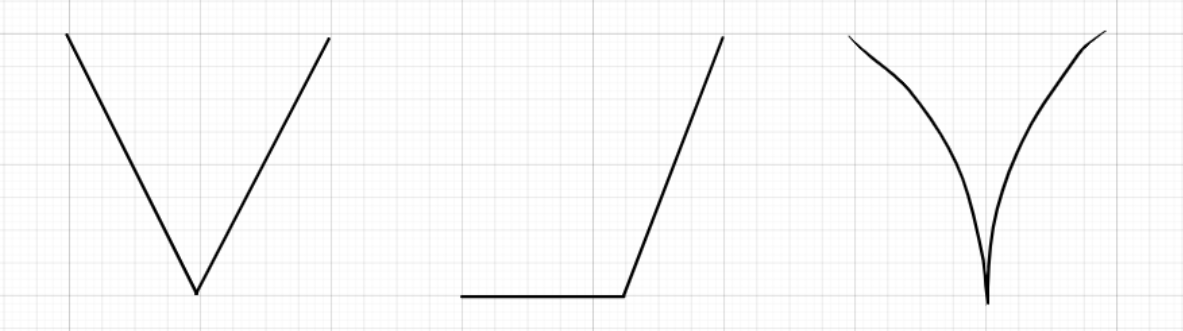
\includegraphics[scale=0.5]{images/img31.png}$$
Точки, в которых функция непрерывна, но не дифференцируема, могут быть исследованы по 1 правилу. Отметим также, что экстремум может достигаться и в точках разрыва функции.
$$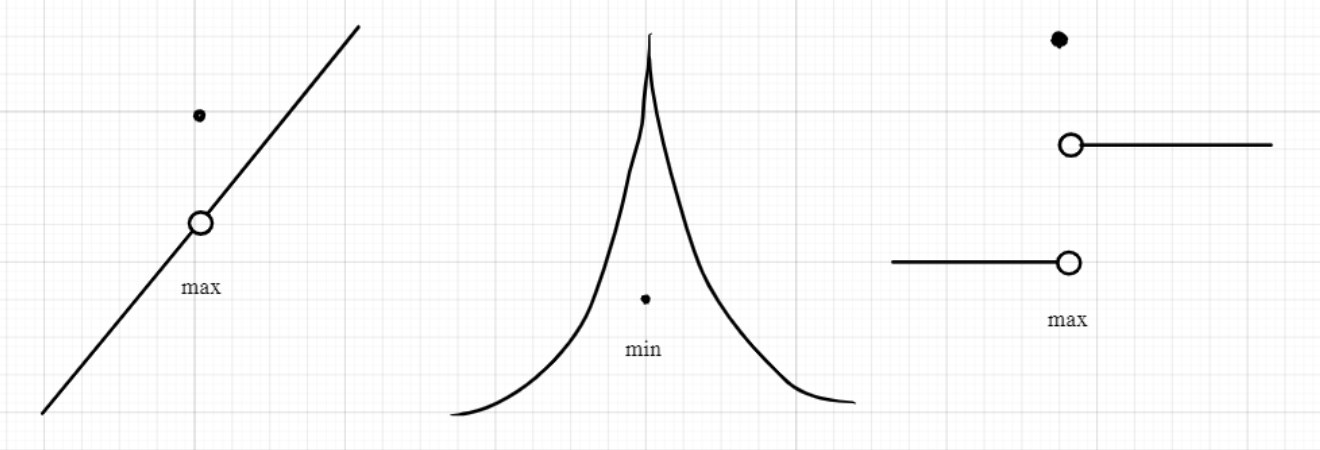
\includegraphics[scale=0.5]{images/img32.png}$$
Точки разрыва исследуются обычно по определению, то есть $f(x_0)$ сравниваются с $f(x)$ для $x \in U(x_0)$. \\
\begin{example}\\ 
	$y = |x|$,  $y = x^{\frac{2}{3}}(1 - x)$ 
\end{example}
\subsection{Глобальный экстремум.}
Зачастую приходится решать задачу о выявлении точек глобального экстремума функции $f$, заданной на множестве $X$ и об определении экстремальных значений функции на всём множестве. Таким образом, нужно найти $x \in X$ (если оно существует) такое, что $f(x) \ge f(x_0)$ (или $f(x) \le f(x_0)$ для $\forall x \in X$).\\\\
Рассмотрим более подробно эту задачу. Сначала выделим случай.
\begin{enumerate}
	\item $f : [a;b] \rightarrow \Rm$, $f \in \mathcal{C}([a;b])$.\\\\
	Из теоремы Вейерштрасса вытекает, что глобальный экстремум в этом случае достигается, то есть $\exists \bar x, \underline{x} \in [a;b]$, такие что $f(\bar x) = \underset{[a;b]}{\max} f$, $f(\underline{x}) = \underset{[a;b]}{\min} f$.\\\\
	Как же найти эти точки? Подумаем, в каких точках может достигаться глобальный экстремум? Из предыдущих рассуждений ясно, что мы должны исследовать ограниченное, вообще говоря, множество точек. А именно: пересмотреть все точки локального экстремума, а также изучить значения $f$ на концах отрезка. Отсюда вытекает последовательность действий при отыскании глобального экстремума функции $f$.
	\begin{enumerate}
		\item Находим все точки возможного локального экстремума функции $f$ на $]a;b[$, то есть точки, в которых $f$ недифференцируема, и стационарные точки $x_1, x_2, \ldots, x_n$;
		\item вычисляем $f(x_1), f(x_2), \cdots, f(x_n)$, а также $f(a), f(b)$;
		\item $\underset{[a;b]}{\max} f = \max \{f(a),f(x_1), f(x_2), \ldots, f(x_n), f(b)\}$;\\
		$ \underset{[a;b]}{\min} f = \min \{f(a),f(x_1), f(x_2), \ldots, f(x_n), f(b)\}$.
	\end{enumerate}
	\item $f: ]a;b[ \rightarrow \Rm, f \in \mathcal{C}(]a;b[)$\\\\
	Это более сложный случай, так как $\underset{[a;b]}{\max} f$ и $\underset{[a;b]}{\min} f$ могут существовать, а могут и не существовать. Однако нетрудно видеть, что задача исследуется до конца в этом случае.\\\\
	Нужно
	\begin{enumerate}
		\item Найти точки возможного экстремума $f$ на $]a;b[$: $x_1, x_2, \ldots, x_n$;
		\item Вычислить $f(x_1), f(x_2), \ldots, f(x_n)$ и добавить $f(a + 0), f(b - 0)$;
		\item Изучить множество $T::=\{f(a + 0),f(x_1), f(x_2), \ldots, f(x_n), f(b - 0)\}$;
		\item Сделать правильные выводы.
	\end{enumerate}
	Если максимальный элемент множества $T$ совпадает с $f(a + 0)$ или $f(b - 0)$, то функция $f$ не обладает глобальным максимумом на $]a;b[$.\\\\
	Если же максимальный элемент один из $f(x_1), f(x_2), \ldots, f(x_n)$, то глобальный максимум есть и мы его нашли. Аналогично исследуется вопрос и для минимума.\\\\
	Этот метод годится и в случае, если $a$ или $b$ есть соответственно символы $-\infty$ или $+\infty$. В этом случае $f(a + 0)$ и $f(b - 0)$ заменяем соответственно символами $f(-\infty)$ и $f(+\infty)$.
\end{enumerate}
Остальные случаи, как-то :$[a;b[, ]a;b]$ принципиально не отличаются от уже рассмотренного и исследуются аналогично (с некоторыми изменениями).
\section{Выпуклые функции.}
\subsection{Определение и глобальный смысл выпуклости.}
$\bullet$ \textit{Фуекцию $f: |a;b| \rightarrow \Rm$ называют \textbf{выпуклой вниз} на промежутке $|a;b|$, если $\forall x_1, x_2 \in |a;b|$ и $\forall \tau \in ]0;1[$ выполняется неравенство
	$$f(x_1 + \tau(x_2 - x_1)) \le f(x_1) + \tau(f(x_2) - f(x_1)).$$}
$\bullet$ \textit{Если в этом неравенстве знак строгий, то $f$ называют \textbf{строго выпуклой вниз}.}\\\\
$\bullet$ \textit{Аналогично, если
	$$f(x_1 + \tau(x_2 - x_1)) \ge f(x_1) + \tau(f(x_2) - f(x_1)),\ \forall x_1, x_2 \in |a;b|,\ \forall \tau \in ]0;1[,$$ то $f$ называют \textbf{строго выпуклой вверх}. }\\\\
Строгое неравенство --- строго выпукла вверх.\\\\
Далее, вместо $"$выпукла вниз$"$ говорим $"$выпукла$"$.
Из определения видно, что если $f$ выпукла, то $-f$ --- выпукла вверх и наоборот, поэтому дальше разговор ведём только о выпуклости. На выпуклые вверх функции результаты легко переносятся.   
\subsection{Геометрический смысл выпуклости.}
Обозначим $x_\tau :: = x_1 + \tau(x_2 - x_1)$.\\\\
Поскольку $0 < \tau <  1$, то $x_\tau$ расположено мeжду $x_1$ и $x_2$ (если $x_1 < x_2 \Rightarrow x_1 < x_\tau < x_2)$.\\\\
Сравним $f(x_\tau)$ с $f(x_1) + \tau(f(x_2) - f(x_1))$.\\
С этой целью напишем уравнение прямой $(AB)$, где $A(x_1;f(x_1))$, $B(x_2;f(x_2))$.
$$Y = f(x_{1}) + (\frac{f(x_{2}) - f(x_{1})} {x_{2} - x_{1}})(X - x_{1}) $$ \\
Найдём значение этой функции в точке X = $x_{i}$ \\
$$Y(x_{i}) = f(x_{1}) + (\frac{f(x_{2}) - f(x_{1})}{x_{2} - x_{1}})(X - x_{1}) = f(x_{1}) + \tau(f(x_{2}) - f(x_{1})) $$ % почему оно не в одну строку ААААААА
Отсюда вытекает, что $f(x_{i}) \leq \Upsilon (x_{i})$. \\\\
Какой же смысл этого неравенства? \\\\
Оно означает, что для любых двух точек на графике выпуклой функции все остальные точки между этими лежат не выше соответствующих точек хорды, стягивающей эти точки графика. Для строго выпуклой функции точки дуги лежат строго ниже соответствующей хорды, стягивающей две произвольные точки графика.
$$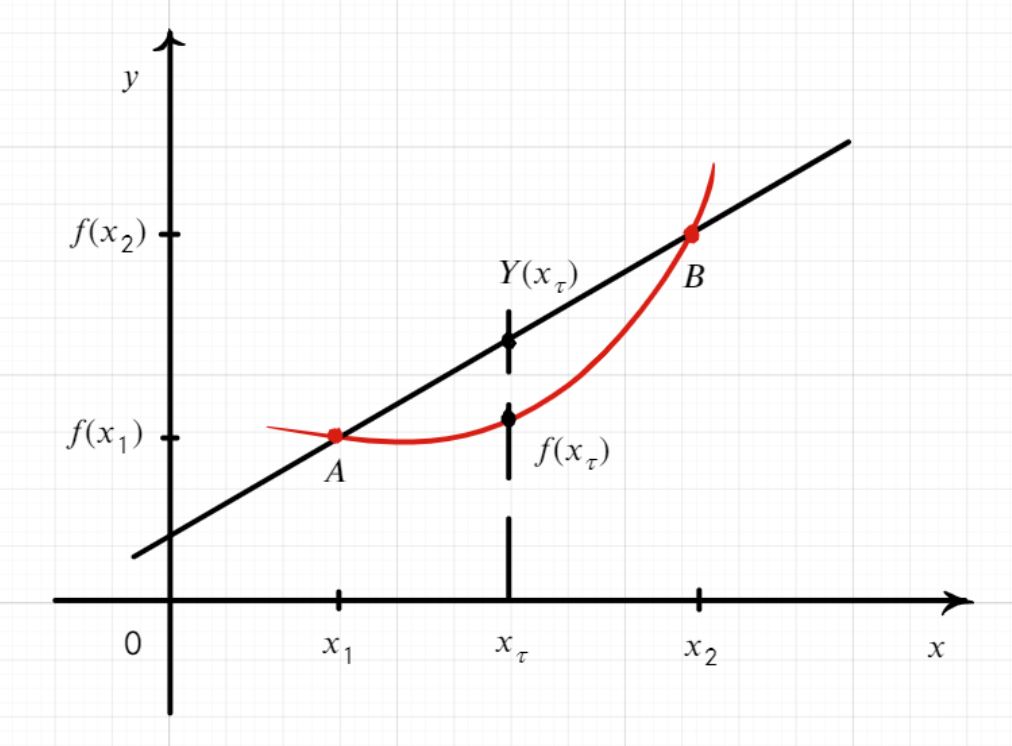
\includegraphics[scale=0.5]{images/img33.png}$$
Для выпуклой вверх функции всё наоборот.
\begin{lem}
	Для выпуклой функции $f$ на $|a;b|$ необходимо и достаточно, чтобы $\forall x_{1}, x_{2} \in |a;b|, x_{1}< x_{2}$ и $\forall x_{1} < x < x_{2}$ выполняется неравенство 
	$$\frac{f(x) - f(x_{1})}{x - x_{1}} \leq \frac{f(x_{2}) - f(x)}{x_{2} - x}$$ 
	(Для строгой выпуклости --- строгое неравенство).
\end{lem} 
\begin{Proof}
	\textbf{Необходимость}. Т.к. $f$ выпукла, то
	$$f(x_{1} + \tau(x_{2} - x_{1})) \leq f(x_{1}) + \tau(f(x_{2}) - f(x_{1}))$$ %тут должно быть i с чертой
	т.к. $x$ --- произвольная точка между $x_{1}$ и $x_{2}$, то
	$\exists \tau \in ]0;1[ $ такое, что $x = x_{1} + \tau(x_{2} - x_{1})$. Oтсюда $\tau = \dfrac{x - x_{1}}{x_{2} - x_{1}}$.
	Тогда условие выпуклости запишется в форме 
	$$f(x) \leq f(x_{1}) + \frac{x - x_{1}}{x_{2} - x_{1}}(f(x_{2}) - f(x_{1})).$$
	Это неравенство можно переписать в форме 
	$$\frac{f(x) - f(x_{1})}{x - x_{1}} \leq \frac{f(x_{1}) - f(x_{2})}{x_{2} - x_{1}}. \eqno(A)$$
	Положим теперь в определении выпуклости $\tau := 1 - \tau, x_{2}: = x_{1}, x_{1}: = x_{2}$ (т. е. поменяем $x_{1}$ и $x_{2}$ ролями)\\
	Тогда $$f(x_{2} + (1 - \tau)(x_{1} - x_{2}))\leq f(x_2)+(1-\tau)(f(x_1)-f(x_2)).$$
	Так как $$tau = \frac{x - x_{1}}{x_{2} - x_{1}} \Ra 1 - \tau = \frac{x_2 - x}{x_{2} - x_{1}}$$
	а также $x_{2} + (1 - \tau)(x_{1} - x_{2}) = x_{1} + \tau(x_{2} - x_{1}) = x$.\\\\
	Поэтому условие выпуклости запишется в виде $$f(x) \leq f(x_{2}) + \frac{x_{2} - x}{x_{2} - x_{1}}(f(x_{1}) - f(x_{2})).$$
	Откуда $$\frac{f(x_{2}) - f(x)}{x_{2} - x} \leq \frac{f(x_{2}) - f(x_{1})}{x_{2} - x_{1}}. \eqno(B)$$
	Из ($А$) и ($В$) $\Ra$
	$$\frac{f(x) - f(x_{1})}{x - x_{1}} \leq \frac{f(x_{2}) - f(x)}{x_{2} - x}$$
	\textbf{Достаточность}. Перепишем неравенство в следующей форме 
	$$(f(x) - f(x_{1}))(x_{2} - x) = (f(x_{2}) - f(x))(x - x_{1})$$
	$$f(x)(x_{2} - x + x - x_{1}) \leq (x - x_{1})f(x_{2}) - (x_{2} - x)f(x_{1})$$
	Представим  $x = x_{1} + \tau(f(x_{2}) - f(x_{1}))$ и получим
	$$f(x_1+\tau(x_2-x_1))\leq f(x_1)+\tau(f(x_2)-f(x_1)),$$
	что и является определением выпуклости.
\end{Proof}\\\\
Геометрически --- это угловые коэффициенты.
$$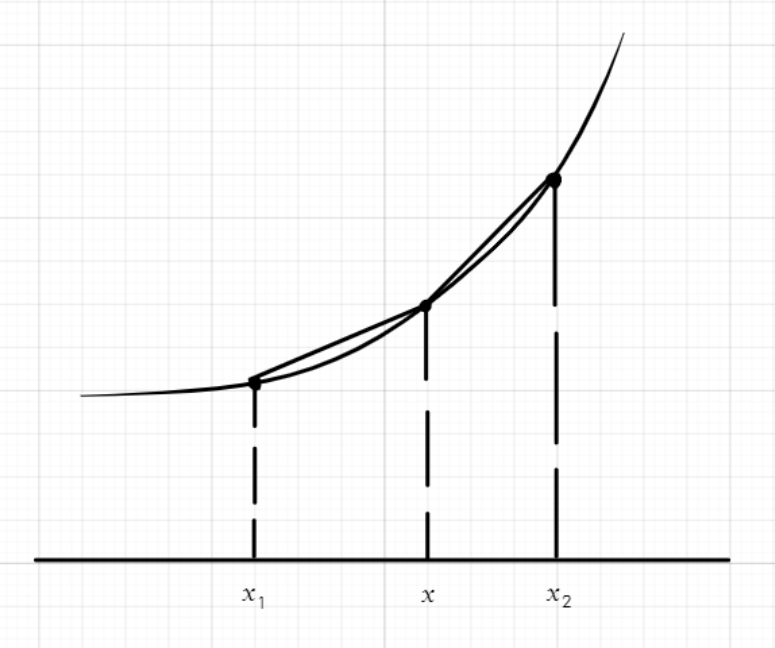
\includegraphics[scale=0.5]{images/img34.png}$$
\begin{theorem}[Критерий выпуклости дифференцируемой функции]
	Для того, чтобы дифференцируемоая на отрезке ]a;b[ $f'$ была возрастающей. При этом строгому возрастанию соответствует строгая выпуклость.
\end{theorem}
\begin{Proof}Для строгой функции.\\
	\textbf{Необходимость}. Пусть $f$ строго выпуклая. Требуется доказать, что $f'(x_{1}) < f'(x_{2}), \forall x_{1}, x_{2}, x_{1} < x_{2}$ \\\\
	В силу леммы: 
	$$\frac{f(x) - f(x_{1})}{x - x_{1}} < \frac{f(x_{2}) - f(x)}{x_{2} - x},\quad \forall x \in ]x_{1};x_{2}[$$
	Перейдём в этом неравенстве к пределу при $x \xrightarrow{} x_{1}$
	$$f'(x_{1}) \leq \frac{f(x_{2}) - f(x_{1})}{x_{2} - x_{1}}$$
	А если в предыдущем неравенстве перейдём к пределу при $x \xrightarrow{} x_{2}$, то получим:
	$$\frac{f(x_{2}) - f(x_{1})}{x_{2} - x_{1}} \leq f'(x_{2})$$
	Из последних двух неравенств следует, что $f'(x_{1}) \leq f'(x_{2})$, т.е. $f'$ --- возрастает (Заметим, что этим уже доказательство закончено для первой части теоремы).\\\\
	Докажем, что возрастание строгое.
	Возьмём $\forall x_{0} \in ]x_{1}; x_{2}[$. По лемме
	$$\frac{f(x_{0}) - f(x_{1})}{x_{0} - x_{1}} < \frac{f(x_{2}) - f(x_{0})}{x_{2} - x_{0}}$$
	Применим формулу конечных приращений $f'(c_{1}) < f'(c_{2})$, где $c_{1} \in ]x_{1};x_{0}[, c_{2} \in ]x_{0};x_{2}[$ \\
	Т. к. $f'$ возрастает, то 
	$f'(x_{1}) \leq f'(c_{1}) < f'(c_{2}) \leq f'(x_{2}) \Ra f'(x_{1}) < f'(x_{2}) \Ra f'$ строго возрастает. \\
	\textbf{Достаточность}. Дано $f'$ строго возрастает. Требуется доказать, что $f$ --- строго выпукла. \\\\
	Возьмём $\forall x_{1}, x_{2}, x \in ]a;b[$ такие что $x_{1} < x < x_{2}$.
	Рассмотрим $\dfrac{f(x) - f(x_{1})}{x - x_{1}} = $ [на основной т. Лагранжа] $= f'(c_{1})$, где $x_{1} < c_{1} < x$.\\\\
	Аналогично $\dfrac{f(x_{2}) - f(x)}{x_{2} - x} = f'(c_{2})$, где $x < c_{2} < x_{2}$.\\\\
	Т.к. $f'(x)$ строго возрастает, то $f'(c_{1}) < f'(c_{2})$, что влечёт за собой 
	$$\frac{f(x) - f(x_{1})}{x - x_{1}} < \frac{f(x_{2}) - f(x)}{x_{2} - x}$$
	И нак основании леммы $\Ra$ $f$ строго выпукла.
\end{Proof}
\begin{cor}
	Пусть $f \in D^2(]a;b[)$. Для выпуклости $f$ на  $]a;b[$ необходимо и достаточно $f''(x) \geq 0$. Для строгой выпуклости необходимо и достаточно $f''(x) \geq 0$ и $f''(x) \not\equiv 0$ ни на одном промежутке из $]a;b[$.
\end{cor}
\begin{Proof}
	Справедливость этих суждений вытекает из критерия выпуклости и критериев монотонности примененённых к $f'$.
\end{Proof}\\
\begin{example}
	$\ln x$ --- строго выпукла вверх.
	$$f'(x) = \frac{1}{x},\quad f''(x) = - \frac{1}{x^2} < 0,\quad \forall x > 0.$$
\end{example}
\subsection{Расположение графика выпуклой функции относительно касательной.}
\begin{theorem}
	Пусть $f \in D(]a;b[)$. Тогда\begin{enumerate}
		\item $f$ выпукла $\Longleftrightarrow$ когда график Г$_{f}$ расположен не ниже касательной к Г$_{f}$ в любой его точке. 
		\item $f$ строго выпукла $\Longleftrightarrow$ когда график Г$_{f}$ расположен выше касательной, проведённой к Г$_{f}$ в любой его точке (за исключением точки касания).
	\end{enumerate}
\end{theorem}
\begin{Proof}
	Для 1.\\\\
	\textbf{Необходимость}. $f$ выпукла. Доказать, какую бы касательную ни взять, то Г$_{f}$ --- не ниже. \\\\
	Возьмём $\forall x_{0} \in ]a;b[$ и напишем уравнение касательной к Г$_{f}$ в точке $(x_{0}, f(x_{0}))$ :
	$$\Upsilon = f(x_{0}) + f'(x_{0})(X - x_{0})$$
	Возьмём $\forall x \neq x_{0}, x \in ]a;b[$ и найдём разность \\\\
	$f(x) - \Upsilon(x) = f(x) - f(x_{0}) - f'(x_{0})(x - x_{0}) =$ [т. Лагранжа] $= f'(c)(x-x_{0}) - f'(x_{0})(x - x_{0}) = (x - x_{0})(f'(c) - f'(x_{0})$,
	где $c$ между $x$ и $x_{0}$.
	$$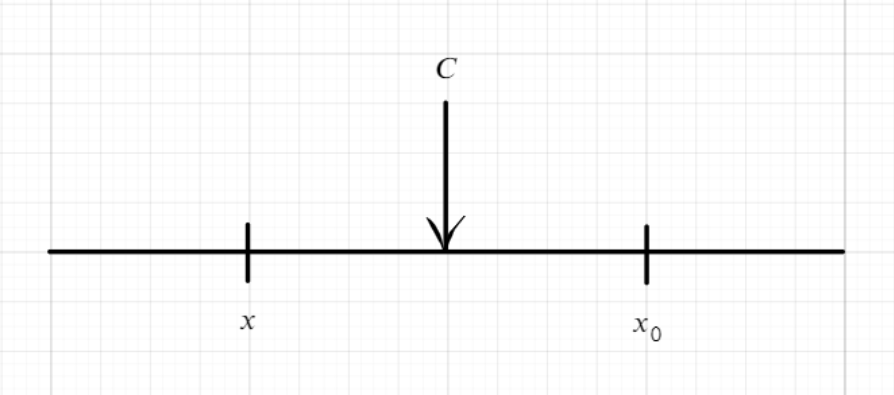
\includegraphics[scale=0.5]{images/img35.png}$$
	Если $x < x_{0}$, то в силу выпуклости $f$ по критерию выпуклости $f'$ возрастает и тогда $f'(c)< f'(c) < f'(x_{0})$, а посему $(x - x_{0})(f'(c) - f'(x_{0})) \geq 0$.\\\\
	Если $x < x_{0}$, то опять $(x - x_{0})(f'(c) - f'(x_{0})) \geq 0$.
	Это означает, что $\forall x_{0} \in ]a;b[, \forall x \in ]a;b[$
	$$f(x) - \Upsilon(x) \geq 0 \implies f(x) \geq \Upsilon(x)$$
	Это означает, что точки графика Г$_{f}$ расположены не ниже соответсвующих точек касательной к Г$_{f}$, проведённой в любой точке.\\\\
	\textbf{Достаточность}. Дано: график не ниже касательной. Требуется доказать, что $f$ выпукла.
	$$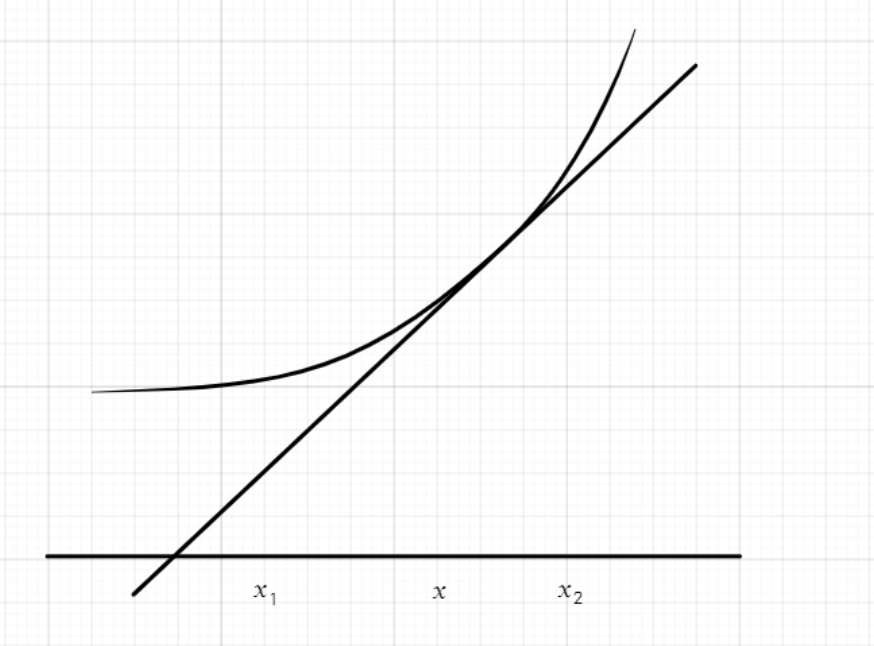
\includegraphics[scale=0.5]{images/img36.png}$$
	Возьмём 3 произвольные точки $x_{1} < x < x_{2}$ и касательную в точке $x_{0}$
	$$f(x) - \Upsilon(x) = f(x) - f(x_{0}) - f'(x_{0})(x - x_{0}) \geq 0 \implies f(x) - f(x_{0} \geq f'(x_{0})(x - x_{0})$$
	Положим здесь $x = x_{1}, x_{0} = x$, тогда $\dfrac{f(x_{1}) - f(x)}{x_{1} - x} \leq f'(x)$.\\\\
	Положим иначе: $x = x_{2}, x_{0} = x$, тогда $\dfrac{f(x_{2}) - f(x)}{x_{2} - x} \leq f'(x)$.\\\\
	Из этих двух последних неравенств следует 
	$$\frac{f(x_{1}) - f(x)}{x_{1} - x} \leq \frac{f(x_{2}) - f(x)}{x_{2} - x}$$
	и по лемме $f$ выпукла.
\end{Proof}
\subsection{Неравенство Йенсена.}
Пусть $f$ выпуклая функция. Тогда $\forall x_{1}, x_{2}$ имеем 
$$f(x_{1} + \tau(x_{2} - x_{1})) \leq f(x_{1}) + \tau(f(x_{2}) - f(x_{1})), \forall \tau \in ]0;1[ $$
$$f((1 - \tau)x_{1} + \tau x_{2}) \leq (1 - \tau)f(x_{1}) + \tau f(x_{2})$$
$$1 - \tau = :: \alpha_{1},\quad \tau = :: \alpha_{2}, \alpha_{1},\quad \alpha_{2} > 0,\quad \alpha_{1} + \alpha_{2} = 1.$$
и получаем: \\
$$f(\alpha_{1}x_{1} +\alpha_{2}x_{2}) \leq \alpha_{1}f(x_{1}) + \alpha_{2}f(x_{2})$$
Последнее неравенство эквивалентно определению выпуклости, и поэтому $f$ выпукла тогда и только тогда, когда для $\forall x_{1}, x_{2}$
$$f(\alpha_{1}x_{1} +\alpha_{2}x_{2}) \leq \alpha_{1}f(x_{1}) + \alpha_{2}f(x_{2}), \forall \alpha_{1}, \alpha_{2};$$
$$0 < \alpha_{1},\quad \alpha_{2} < 1,\quad \alpha_{1} + \alpha_{2} = 1.$$
$\bullet$ \textit{Это и есть \textbf{неравенство Йенсена}.} \\\\
Индукцией по $n$ оно переносится и на большее число слагаемых. \\\\
$f$ выпукла $\Ra \forall x_{1}, x_{2}, \ldots, x_{n},\ n > 2$ 
$$f(\alpha_{1}x_{1}, \alpha_{2}x_{2},\ldots, \alpha_{n}x_{n}) \leq \alpha_{1}f(x_{1}), \alpha_{2}f(x_{2}),\ldots, \alpha_{n}f(x_{n})$$
$$0 < \alpha_{i} < 1,\quad \sum_{i=1}^{n}\alpha_{i} = 1.$$
\begin{example}
	$\ln$ --- строго выпуклая вверх функция. Поэтому на основаниии неравенства Йенсена \\
	$$\ln(\alpha_{1}x_{1}, \alpha_{2}x_{2},\ldots, \alpha_{n}x_{n}) \geq \alpha_{1}\ln(x_{1}), \alpha_{2}\ln(x_{2}),\ldots, \alpha_{n}\ln(x_{n})$$
	Потенцируем
	$$\alpha_{1}x_{1}, \alpha_{2}x_{2} ,\ldots, \alpha_{n}x_{n} \geq x_{1}^{\alpha_{1}} \cdot x_{2}^{\alpha_{2}} \cdot \ldots \cdot x_{n}^{\alpha_{n}}$$
	Положим здесь $\alpha_{\beta} = \dfrac{1}{n};\ 0 < \dfrac{1}{n} < 1,\ \sum\limits_{\beta=1}^{n} = \dfrac{1}{n}= \dfrac{1}{n} \cdot n = 1$.
	$$\frac{x_{1} + x_{2} + \ldots + x_{n}}{n} \geq \sqrt[n]{x_{1}\cdot x_{2}\cdot\ldots\cdot x_{n}}$$
	Среднее арифмитическое $n$ чисел больше или равно среднему геометрическому этих же чисел.
\end{example}
\section{Исследование функций.}
\subsection{Точки перегиба.}
$\bullet$ \textit{Пусть $f: U(x_{0}) \to R$ --- функция, определённая и дифференцируемая в окрестности $\dot{U}(x_{0})$ точки $x_{0}$, причем в самой точке конечная и бесконечная производные. Если на множествах $ \dot{U}_-(x_{0})$ и $\dot{U}_+(x_{0})$ функция $f$ имеет различные направления выпуклости, то точка $(x_{0}, f(x_{0}))$ графика Г$_f$ называется его \textbf{точкой перегиба}. Иногда говорят что $x_{0}$ --- \textbf{точка перегиба} функции.} \\\\
Таким образом, вспоминая расположение графика выпуклой функции относительно касательной, заключаем, что в точке перегиба $(x_{0}, f(x_{0}))$ график Г$f$ переходит с одной стороны касательной на другую, т.е. расположены по разные стороны касательной.
$$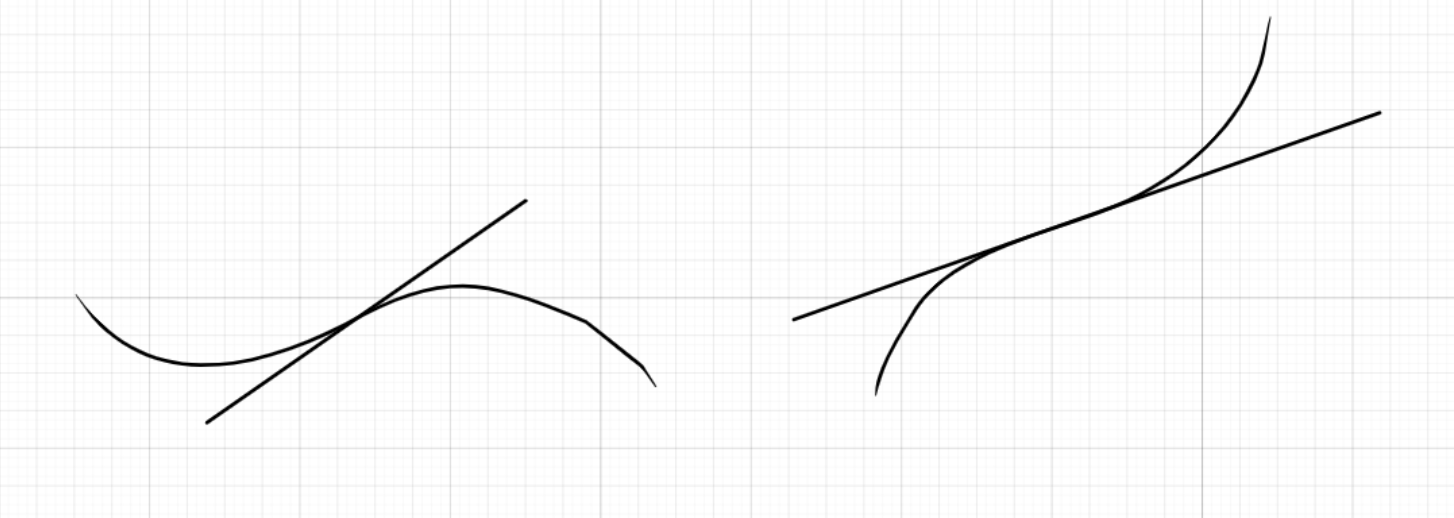
\includegraphics[scale=0.5]{images/img37.png}$$
\begin{theorem}
	Необходимым условием точки перегиба дважды дифференцируемой функции является условие $f''(x_{0}) = 0$.
\end{theorem}
\begin{Proof}
	Пусть $(x_{0}, f(x_{0}))$ --- точка перегиба графика Г$_f$. Тогда на $ U_-(x_{0})$ и $U_+(x_{0})$ функция $f$ выпукла в различных смыслах, и, следовательно, на этих промежутках, согласно критерию выпуклости монотонна в противоположных смыслах $x_{0}$ --- точка локального экстремума для $f'$, и, значит, $x_{0}$ --- стационарная точка для $f'$: $(f')'(x_{0}) = 0 \Ra f''(x_{0})$.
\end{Proof}\\\\
\textit{Таким образом, точками возможного перегиба дважды дифференцируемой функции являются точки, в которых $f$ обращается в нуль.} \\\\
$\bullet$\textit{ Такие точки называются точками \textbf{распрямления}.} \\\\
\textit{Кроме того, подлежат исследованию точки в которых $f''$ не существует.}
\subsection{Достаточные условия точки перегиба.}
Пусть $(x_{0}, f(x_{0}))$ --- точка, в которой возможен перегиб. Т.к. точки перегиба являются точками локального экстремума для $f'$, что достаточно переформулировать 3 правила локального экстремума для $f$ применительно к $f'$. При этом не нужно учитывать максимум в точке или минимум для $f'$. \\
\begin{enumerate}
	\item  \textit{Пусть $f \in D^2(\dot{U}(x_{0}))$. Если $f''$ при переходе через точку $x_{0}$ меняет знак, то $(x_{0}, f(x_{0}))$ --- точка перегиба. Если $f''$ знак не меняет, то $(x_{0}, f(x_{0}))$ не является точкой перегиба.} \\
	\item \textit{Пусть $f \in D^3(\dot{U}(x_{0}))$ и $f''(x_{0}) = 0$. Если $f'''(x_{0}) \neq 0$, то $(x_{0}, f(x_{0}))$ --- точка перегиба.} \\
	\item \textit{Пусть и $f \in D^n(\dot{U}(x_{0}))$ и $f''(x_{0}) = \ldots = f^{(n-1)}(x_{0}) = 0$, а $f^{(n-1)}(x_{0}) \neq 0$. Тогда если $n$ --- нечётно, то  $(x_{0}, f(x_{0}))$ --- точка перегиба, если $n$ --- чётно, то  $(x_{0}, f(x_{0}))$ не является точкой перегиба.}
\end{enumerate}
\begin{example}
	\begin{enumerate}
		\item $f(x) = ax + \sin{x}$; $f''(x) = -\sin{x} = 0 \Ra x = k\pi$ --- точка рассчёта. $f'''(x) = -\cos{k\pi} \neq 0 \Ra x = k\pi$ --- точка перегиба.
		\item $f(x) = \sqrt[3]{x^4}$; $f'' = \frac{4}{9}x^-\frac{2}{3}$ в точке $x = 0$  $f''$ не существует, т.к. $f''$ не меняет знак, то $x_{0} \neq 0$ не является точкой перегиба.
	\end{enumerate}
\end{example}
\subsection{Асимптоты}
$f: \dot{U}(x_{0}) \to R$. Пусть $c \in X$ либо является граничной точкой множества $X$ (концов одного из промежутков, составляющих $X$), причём $c \in R, c \neq \pm \infty$. \\\\
$\bullet$ \textit{Если $\exists \lim\limits_{x \to c+0}f(x) = \infty$, то прямая $x=c$ называется \textbf{правосторонней вертикальной асимптотой} графика Г$f$ функции $f$.} \\\\
$\bullet$ \textit{Если $\exists \lim\limits_{x \to c-0}f(x) = \infty$, то $x=c$ --- \textbf{левосторонняя вертикальная асимптота}.} \\\\
$\bullet$ \textit{Если $\exists \lim\limits_{x \to c}f(x) = \infty$, то $x=c$ --- \textbf{двусторонняя вертикальная асимптота}.} \\\\
Мы найдём все вертикальные асимптоты, если исследуем точки, в которых функция терпит разрыв, или точки, не принадлежащие $X = D(f)$, но являющиеся граничными для $D(f)$.\\
\begin{example}
	$y = \dfrac{1}{\sqrt{x}}$, $ x = 0$ --- правосторонняя вертикальная асимптота, $y = \dfrac{1}{x+2}$, $x = -2$ --- двусторонняя вертикальная асимптота.
\end{example}\\\\
Предположим, что $X$ содержит промежуток $[a;+\infty[$. \\\\
$\bullet$ \textit{Прямая $y = kx + b$, где $k,b \in \Rm$ называется \textbf{наклонной асимптотой} для Г$_f$ \textbf{вправо}, если $$\lim\limits_{x \to + \infty}f(x) - (kx+b) = 0 \eqno(*)$$ или, в равносильной форме
	$$f(x) - (kx+b) = o(1),$$  при $x \to +\infty$.}\\\\
$\bullet$\textit{ Аналогично, если в $D(f)$ входит промежуток $]-\infty; \beta|$, и $f(x) - (kx+b) = o(1), \quad x \rightarrow +\infty$, то $y = kx +b$ называют \textbf{наклонной асимптотой влево}}.\\\\
$\bullet$ \textit{Если же $f(x) - (kx+b) = o(1)$ при $x \rightarrow \infty$, то $y = kx +b$ --- \textbf{двусторонняя наклонная асимптота}.}\\\\
Как же обнаружить наклонные асимптоты, то есть как найти $k$ и $b$ ?\\\\
$\underset{x \rightarrow +\infty}{\lim}{(f(x)-(kx+b))} = \underset{x \rightarrow +\infty}{\lim}{x(\frac{f(x)}{x}-k - \frac{b}{x})} = 0
\Rightarrow \underset{x \rightarrow +\infty}{\lim}{(\frac{f(x)}{x} - k - \frac{b}{x})} = 0 \Rightarrow$  $$\boxed{k = \underset{x \rightarrow +\infty}{\lim}{\frac{f(x)}{x}}}$$
Если $k$ существует, то точка $$\boxed{b = \underset{x \rightarrow +\infty}{\lim}{(f(x) - kx)}}.$$
Определив таким образом $k$ и $b$, мы находим наклонную асимптоту вправо: $y = kx+ b$ --- её уравнение аналогично наклонной асимптоте влево; те же формулы но при $x \rightarrow -\infty$.\\\\
Обычно пытаются найти указанные  пределы при $x \rightarrow \infty$. Если они существуют, то $y = kx +b$ --- двусторонняя наклонная асимптота.\\\\
При отыскании наклонных асимптот широко используют правило Лопиталя:\\\\
Например, $f(x) \rightarrow \infty$  при $x \rightarrow \infty$ и $\exists\underset{x \rightarrow \infty}{\lim}{f^{'}(x)}$.
Тогда $k = \underset{x \rightarrow \infty}{\lim}{\dfrac{f(x)}{x}} = \underset{x \rightarrow \infty}{\lim}{f^{'}(x)}$.
\subsubsection{Геометрический смысл асимптот.}
Асимптота, согласно определению, это такая прямая, что расстояние от точки на ней до кривой $f$ стремится к нуля при $x \rightarrow \infty$. Таким образом, асимптотами можно заменять для достаточно больших значений аргумента участок графика функции.\\\\
Для некоторых функции одна прямая является двусторонней асимптотой, для других разные асимптоты вправо и влево. Может быть только вправо, только влево, а то и вовсе не быть.\\\\
Среди наклонных асимптот выделяют иногда горизонтальные асимптоты. Как видно из полученных выше формул, если 
$\exists \underset{x \rightarrow \infty}{\lim}{f(x)} = b$, то $ y = b$ --- горизонтальная асимптота.\\
\begin{example}\\
	$y = x \arctan{x} \quad \mathbb{D} = \Rm$\\
	$k = \underset{x \rightarrow \pm\infty}{\lim}{\arctan{x}} = \pm \frac{\pi}{2}$\\
	$b = \underset{x \rightarrow +\infty}{\lim}{(x\arctan{x} - x \frac{\pi}{2})} = \underset{x \rightarrow +\infty}{\lim}{\dfrac{\arctan{x} - \frac{\pi}{2}}{\frac{1}{x}}} = \underset{x \rightarrow +\infty}{\lim}{\dfrac{\frac{1}{1+x^2}}{-\frac{1}{x^2}}} = -1;\\\\
	y = \dfrac{\pi}{2}x -1$ --- наклонная асимптота вправо\\
	$y = -\dfrac{\pi}{2}x-1$ --- наклонная асимптота влево.
\end{example}
\section{Характерные точки $f$.} 
Пусть функция задана на $X$, состоящем из конечного или бесконечного числа промежутком действительной оси, причём, если промежутков бесконечно много, то предполагаем, что на каждом ограниченном отрезке располагается лишь конечное число промежутков их $X$.\\
\textbf{\textit{Характерными точками $f$ будем называть:}}
\begin{enumerate}
	\item \textit
	{
		Точки, не входящие в $X$, но являющегося конечным хотя бы одного из промежутков $X$. 
	}
	\item \textit
	{
		Точки разрыва $f$. 
	}
	\item \textit
	{
		Точки не дифференцируемости $f$,То есть точки, где либо $f'$ не существует либо $f' = \infty$.
	}
	\item \textit
	{
		Стационарные точки $(f' = 0)$.
	}
	\item \textit
	{
		Точки, где $f''$ не существует, либо $f'' = \infty$. 
	}
	\item \textit
	{
		Точки расправления $(f'' = 0)$.
	}
	\item \textit
	{
		Точки, исключительные по какому-нибудь другому признаку, например, нули функции и другое
	}
\end{enumerate}
При построении графиков функций выделяют участки единообразного поведения функции, то есть участки, на которых $f'$ и $f''$ существуют, непрерывны и сохраняют знак. На каждом из таких участков функция строго монотонна и имеет определённое направление выпуклости. Кроме того, к участкам единообразного поведения функции причисляем участки постоянства функции. Участки единообразного поведения функции обычно разделяются характерными точками.
\section{Схема построения графика.}
\begin{enumerate}
	\item Определяем мнодество задания функции. Исследуем функцию на периодичность и четность. Если функция периодична, то строим график функции $f$ на промежутке равном длине периода. Если $f$ четна, либо нечетна, то строим график Г$_f$ для $x\geq 0$ и далее используем симметрию.
	\item Выделяем участки непрерывности, определяем характер точек разрыва. Находим вертикальные асимптоты. Находим предельные значения функции при стремлении $x$ к граничным точкам множества задания, в том числе и к $\pm \infty$, если функция позволяет это сделать. Если $\exists\lim\limits_{x\to\infty} f(x) = a$, то $y = a$ --- горизонтальная асимптота.
	\item Находим наклонные асимптоты.
	\item Находим $f^\prime$. Определяем критические точки и выявляем их характер. Промежутки возрастания и убывания.
	\item Находим $f^{\prime\prime}$. Точки распрямления. Точки, где $f^{\prime\prime}$ не существует или бесконечна. Определяем точки перегиба и направления выпуклости.
	\item Составляем таблицу. В $I$ графе --- участки единообразного поведения функции и характерные точки. Во $II$ и $III$ --- знаки производных и их значения. В $IV$ --- эскиз графика на заданном участке.
	\item Вычисляем значения $f$ в случайных точках, точки пересечения с осями, выясняем близость $f$ с кривыми более простой структуры и так далее.
	\item Наносим всё на чертёж и строим график.
\end{enumerate}
%
%
% 218-221
%
%